\sectioncounter{6}
  \section{二次函数}

  \subsection{知识梳理}
  形如 $y=ax^2+bx+c$ ($a\neq 0$) 的函数称为\myindex{二次函数} (quadratic function), 其图象为抛物线. 二次函数的系数对图象的影响有:
  
  (1) $a$ 的正负号决定开口方向, 绝对值决定开口大小 (形状);
  
  (2) 对称轴为直线 $x=-\dfrac{b}{2a}$;
  
  (3) 判别式 $\Delta= b^2-4ac$ 的符号决定图象与 $x$~轴交点的个数;
  
  (4) $(0,c)$ 为图象与 $y$~轴交点, 即 $c$ 为纵截距.
  
  除 $y=ax^2+bx+c$ (\myemph{一般式}) 外, 二次函数解析式还可以改写为 
  \mymarginpar{解题时应根据已知条件选择合适的解析式形式.}
  \begin{align*}
    &y=a(x-h)^2+k\text{\quad(\myemph{顶点式})},\\
    &y=a(x-x_1)(x-x_2)\text{\quad(\myemph{两根式})}.
  \end{align*}
  画二次函数图象时, 常把一般式通过配方化为顶点式, 
  解二次方程或二次不等式时, 常把一般式通过因式分解 (如十字相乘法) 化为两根式.
  由二次函数的图象可以直接得到对应二次方程和二次不等式的解集. 
  
  设二次函数 $y=ax^2+bx+c$ 与 $x$~轴交于 $(x_1,0)$, $(x_2,0)$, 则
  \[\left\{\!\!\begin{array}{l}
      x_1+x_2=-\dfrac{b}a,\\
      x_1x_2=\dfrac{c}a,
    \end{array}\right.\quad
    \text{且\ }|x_1-x_2|=\frac{\sqrt{\Delta}}{|a|}.\]
  上面前一组公式也称为\myindex{韦达定理}或\myindex{根与系数关系}, 
  \mymarginpar{\myemph{韦达定理的推导}: 把两根式展开
    %\[y=ax^2-a(x_1+x_2)x+ax_1x_2,\]
    和一般式对比, 或由求根公式直接验证.}
  后一个公式为两根之间的距离公式, 可由韦达定理或求根公式推得.
  在解决二次方程的根的分布问题时, 主要考虑二次函数的对称轴、判别式和所选区域的端点值.

  \lianxi
  \begin{exercise}
    函数 $f(x)=x^2$, $x\in [-1,2)$ 的最小值为\,?
    \mymarginpar{$f(x)$ 在 $[-1,2)$ 上不是单调函数, 最值不是端点值.}
  \end{exercise}

  \beginsolution
    $f_{\min}=f(0)=0$.
  \endsolution
  
  \begin{exercise}
    若函数 $f(x)=x^2 -2ax+2a+4$ 的值域为 $[1,+\infty)$,
    求实数 $a$ 的值.
  \end{exercise}

  \beginsolution
    方法一: $f(x)=x^2 -2ax+2a+3\geqslant 0$ 恒成立, 且 ``$=$'' 可以取到, 则 $(2a)^2-4(2a+3)=0$, 解得 $a=-1$ 或 $3$.
    
    方法二: $f(x)=(x-a)^2-a^2+2a+4$ 或由轴为 $x=a$ 知
    \[f_{\min}=f(a)=-a^2+2a+4=1,\]
    解同上.
    
    \varexercise $f(x)$ 不变, 记 $g(a)=f_{\min}$, 求 $g_{\max}$.
    
    由 $g(a)=f(a)=-a^2+2a+4$ 知 $g_{\max}=g(1)=5$.
  \endsolution
  
  \begin{exercise}
    若关于 $x$ 的方程 $x^2 +mx+1=0$ 有两个不相等的实数根, 
    则实数 $m$ 的取值范围是\,?
  \end{exercise}

  \beginsolution
    $\Delta=m^2-4\cdot1>0$, 解得 $m\in(-\infty,-2)\cup(2,+\infty)$.
  \endsolution
  
  \begin{exercise}
    设函数 $f(x)=\begin{cases}  
      -2, & x>0,\\
      x^2+bx+c, & x\leqslant 0,
    \end{cases}$ 若 $f(-4)=f(0)$, $f(-2)=0$, 
    则 $f(x)\leqslant 1$ 的解集为\,?
  \end{exercise}

  \beginsolution
    二次函数图象的轴为 $x=-2=-\frac{b}2$, 则 $b=4$. 由 $f(-2)=0$ 解得 $c=4$. 分类讨论可得所求解集为 $[-3,-1]\cup(0,+\infty)$.
  \endsolution
  
  \subsection{要点导学\quad 各个击破}
  \subsubsection{求二次函数的解析式}
  \begin{example}
    已知函数 $f(x)=ax^2+bx+c$, 关于 $x$ 的不等式 $f(x)>-2x$ 的解集为 $(1,3)$, 
    且方程 $f(x)+6a=0$ 有两个相等的实数根, 求 $f(x)$ 的解析式.
  \end{example}

  \beginsolution
    不等式化为 $ax^2+(b+2)x+c>0$, 则 $a<0$ 且
    \[\left\{\!\!\begin{array}{l}
        \frac{c}a= 1\cdot 3,\\
        -\frac{b+2}a= 1+3,
      \end{array}\right.\quad\text{即\ }
      \left\{\!\!\begin{array}{l}
        b=-4a-2,\\
        c=3a.
      \end{array}\right.\]
    方程化为 $a^2+bx+c+6a=0$, 则 $b^2-4a(c+6a)=0$.
    联立解得 $a=-\frac15$, $b=-\frac65$, $c=-\frac35$. 故
    $f(x)=-\frac15(x^2+6x+3)$.
  \endsolution
  
  \begin{example}
    已知函数 $f(x)=ax^2 +bx+c$ ($a\neq 0$) 满足 $f(0)=-1$, 
    对任意的 $x\in \mathbb{R}$ 都有 $f(x)\geqslant x-1$,
    且 $f\Bigl(-\dfrac12+x\Bigr)= f\Bigl(-\dfrac12-x\Bigr)$, 
    求函数 $f(x)$ 的解析式.
  \end{example}

  \beginsolution
    $c=-1$, 不等式化为 $ax^2+(b-1)x\geqslant 0$, 则 $b=1$. 又有 $f(x)$ 的轴为 $x=-\frac12=-\frac{b}{2a}$, 故 $a=1$, $f(x)=x^2+x-1$.
  \endsolution
  
  \lianxi
  \begin{exercise}
    若二次函数图象的顶点是 $(1,-3)$, 且过点 $P(2,0)$, 求其解析式.
  \end{exercise}

  \beginsolution
    设 $f(x)=a(x-1)^2-3$, 把 $(2,0)$ 代入知 $a=3$.
  \endsolution
  
  \begin{exercise}
    已知二次函数 $f(x)=x^2 -2bx+a$ 满足 $f(x)=f(2-x)$,
    \mymarginpar{$\phantom{\Leftrightarrow{}}f(x)=f(m-x)$\\
      $\Leftrightarrow f(x)$ 有对称轴 $x=\frac{m}2$;\\
      $\phantom{\Leftrightarrow{}}f(n+x)=f(m-x)$\\
      $\Leftrightarrow f(x)$ 有对称轴 $x=\frac{m+n}2$.}
    且方程 $f(x)-\dfrac{3a}4=0$ 有两个相等的实数根, 
    求函数 $f(x)$ 的解析式.
  \end{exercise}

  \beginsolution
    轴为 $x=1$, 则 $b=1$, 方程化为 $x^2-2x+\frac{a}4=0$, 则 $a=4$.
  \endsolution

  \subsubsection{二次函数的图象和性质}
  \begin{example}
    已知 $a\in \mathbb{R}$, 函数 $f(x)=x^2 -2ax+5$.
    
    (1) 若 $f(x)>0$ 对任意的 $x\in (0,+\infty)$ 恒成立,
    求 $a$ 的取值范围;
    
    (2) 若 $a>1$, 且函数 $f(x)$ 的定义域和值域均为 $[1,a]$, 求 $a$ 的值.
  \end{example}

  \beginsolution
    (1) 对 $x>0$, $f(x)>0$ 化为 $2a<x+\frac5x$, 则
    \mymarginpar{此方法为 ``分离参数法''. ``$f(x)>0$ 恒成立'' 也可以直接化为 ``$f_{\min}>0$''.}
    \[2a<\Big(x+\frac5x)_{\min}=2\sqrt5,\text{\ 即\ }
      a\in(-\infty,\sqrt5).\]
    
    (2) $f(x)=(x-a)^2+5-a^2$, 轴为 $x=a$, 在 $[1,a]$ 上 $\searrow$, 则 $f(1)=a$, $f(a)=1$, 解得 $a=2$.
    
    \varexercise 设  $f(x)=x^2-4x+5$, 是否存在 $m$, $n$ ($m<n$) 使得 $f(x)$ 的定义域和值域均为 $[m,n]$.
    
    $f(x)$ 轴为 $x=2$. 若 $m<n\leqslant 2$, 则 $f(x)$ 在 $[m,n]$ 上 $\searrow$, $f(m)=n$ 且 $f(n)=m$, 作差得 $m+n=3$. 回代解得 $m=1$, $n=2$.
    
    若 $m\leqslant 2< n$, 则 $f(x)$ 在 $[m,2]$ 上 $\searrow$, $(2,n]$ 上 $\nearrow$, $f_{\min}=f(2)=m$ 即 $m=1$. 此时若 $n\in(2,3]$, 则 $f_{\max}=f(1)=n$ 即 $n=2$, 矛盾; 若 $n\in(3,+\infty)$, 则 $f_{\max}=f(n)=n$, 解得 $n=\frac{5+\sqrt5}2$.
    
    若 $2<m<n$, 则 $f(x)$ 在 $[m,n]$ 上 $\nearrow$, $f(m)=m$ 且 $f(n)=n$, 解得 $m=n=\frac{5+\sqrt5}2$, 矛盾.
    
    综上知, 存在合题意的 $m$, $n$ 且 $m=1$, $n=2$ 或 $\frac{5+\sqrt5}2$.
  \endsolution
  
  \lianxi
  \begin{exercise}[s]
    已知函数 $g(x)=ax^2 -2ax+1+b$ ($a>0$) 在 $[0,3]$ 
    上有最大值 $5$ 和最小值 $1$, 求 $a$, $b$ 的值.
  \end{exercise}

  \beginsolution
    $g(x)=a(x-1)^2+1+b-a$, 则 $g(1)=1$, $g(3)=5$, 解得 $a=b=1$.
  \endsolution
  
  \subsubsection{一元二次方程实根的分布问题}
  \begin{example}
    若关于 $x$ 的方程 $x^2 +2kx-1=0$ 的两根 $x_1$, $x_2$ 
    满足 $-1\leqslant x_1 <0<x_2 <2$, 求 $k$ 的取值范围.
  \end{example}

  \beginsolution
    设 $f(x)=x^2+2kx-1$, 则
    \[f(-1)\geqslant 1,\quad f(0)<0,\quad f(2)>0,\]
    \mymarginpar{\centering
    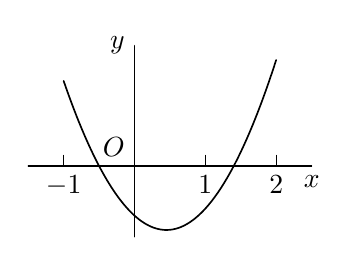
\begin{tikzpicture}[line cap=round,line join=round,scale=0.9]
      \draw[\myaxisarrow] (-1.5,0) -- (2.5,0) node[below] {$x$};
      \draw[\myaxisarrow] (0,-1) -- (0,1.7) node[left] {$y$};
      \draw[line width=0.6pt,smooth,samples=100] 
        plot[domain=-1:2](\x,{(\x+0.5)*(\x-1.4)});
      \draw (0,0) node[anchor=south east] {$O$} 
        (-1,0) node[below] {$-1$}--(-1,0.15) 
        (1,0) node[below] {$1$}--(1,0.15)
        (2,0) node[below] {$2$}--(2,0.15);
    \end{tikzpicture}}
    解得 $k\in\Bigl(-\frac34,0\Bigr]$.
  \endsolution
  
  \subsubsection{课堂评价}
  \begin{exercise}
    已知函数 $f(x)=2x^2 -mx+3$ 在 $(-\infty ,-1)$ 上单调减, 
    在 $(-1,+\infty )$ 上单调增, 那么实数 $m=$\,?
  \end{exercise}

  \beginsolution
    轴 $x=-1$, 可知 $m=-4$.
  \endsolution
  
  \begin{exercise}
    函数 $f(x)=2x^2 -6x+1$ 在区间 $[-1,1]$ 上的最小值为\,? 最大值为\,?
  \end{exercise}

  \beginsolution
    轴 $x=\frac32$, $f_{\min}= f(1)=-3$, $f_{\max}= f(-1)=9$.
  \endsolution
  
  \begin{exercise}
    已知关于 $x$ 的不等式 $ax^2 -bx-1\geqslant 0$ 的解集是 $[2,3]$, 
    那么关于 $x$ 的不等式 $x^2 -bx-a<0$ 的解集是\,?
  \end{exercise}

  \beginsolution
    关于 $x$ 的方程 $ax^2 -bx-1=0$ 的两根为 $2$, $3$ 且 $a<0$, 可解出 $a=-\frac16$, $b=-\frac56$. 再解后一不等式得 $x\in\Bigl(-\frac12,-\frac13\Bigr)$.
  \endsolution
  
  \begin{exercise}
    对于任意实数 $x$, 函数 $f(x)=(5-a)x^2 -6x+a+5$ 恒为正值, 
    则 $a$ 的取值范围是\,?
  \end{exercise}

  \beginsolution
    若 $5-a=0$, 则 $f(x)=-6x+10$, 不合题意. 
    \mymarginpar{此题不宜用分离参数法.}
    所以 $5-a>0$, 利用判别式为负解得 $a\in(-4,4)$.
  \endsolution
  
  \subsection{课后练习}
  \begin{exercise}
    若函数 $y=x^2 +mx+1$ 的最小值为 $0$, 则实数 $m=$\,?
  \end{exercise}

  \beginsolution
    函数图象与 $x$~轴相切, 所以 $m^2-4\cdot 1=0$, $m=\pm2$.
  \endsolution
  
  \begin{exercise}
    函数 $f(x)=2x^2 -4x+1$ 在区间 $[-1,4]$ 上的最小值是\,? 最大值是\,?
  \end{exercise}

  \beginsolution
    轴 $x=1$, $f_{\min}=f(1)=-1$, $f_{\max}=f(4)=17$.
  \endsolution
  
  \begin{exercise}
    已知二次函数的图象经过点 $A(1,2)$, $B(0,-7)$, 对称轴方程为 $x=2$,
    那么其解析式为\,?
  \end{exercise}

  \beginsolution
    用顶点式容易求得解析式为 $y=-3(x-2)^2+5$.
  \endsolution
  
  \begin{exercise}
    若函数 $y=x^2 +(a+2)x+3$, $x\in [a,b]$ 的图象关于直线 $x=1$ 对称,
    则实数 $b=$\,?
  \end{exercise}

  \beginsolution
    轴 $x=-\frac{a+2}2=1$ 且 $\frac{a+b}2=1$, 解得 $a=-4$, $b=6$.
  \endsolution
  
  \begin{exercise}
    若函数 $f(x)=x^2 -2x+2$ 的定义域和值域均为 $[1,b]$ ($b>1$), 则 $b=$\,?
  \end{exercise}

  \beginsolution
    $f_{\max}=f(b)=b$, 解得 $b=1$ (舍) 或 $2$.
  \endsolution
  
  \begin{exercise}
    已知函数 $f(x)=ax^2 +bx+1$ ($a>0$, $b\in \mathbb{R}$) 
    的最小值是 $f(-1)=0$, $F(x)=\begin{cases}
      f(x), & x>0,\\ -f(x), & x<0,\end{cases}$
    则 $F(3)+F(-4)$ 的值为\,?
  \end{exercise}

  \beginsolution
    轴 $x=-1$ 且 $f(-1)=0$, 解得 $a=1$, $b=2$, 所以 
    \[F(3)+F(-4)= f(3)-f(-4)=7.\]
  \endsolution
  
  \begin{exercise}
    若函数 $f(x)=ax^2 +2(a+1)x+2$ 在 $(-\infty,4) $上是增函数,
    则实数 $a$ 的取值范围是\,?
  \end{exercise}

  \beginsolution
    若 $a=0$, 则 $f(x)=2x+2$, 合题意. 若 $a\neq0$, 则必有 $a<0$ 且 $-\frac{2(a+1)}{2a}\geqslant 4$, 解得 $a\geqslant -\frac15$.
    
    综上知, $a\in\Bigl[-\frac15,0\Bigr]$.
  \endsolution
  
  \begin{exercise}
    已知定义域为 $\mathbb{R}$ 的函数 $f(x)$ 满足 $f(x+1)=2f(x)$,
    且当 $x\in [0,1]$ 时, $f(x)=4x^2 -4x$, 那么当 $x\in [-2,-1]$ 时,
    $f(x)$ 的最小值为\,?
  \end{exercise}

  \beginsolution
    方法一: $x\in[0,1]$ 时, $f_{\min}=f\Big(\frac12\Big)=-1$. 
    \mymarginpar{$f(x)$ 图象如下
    \begin{center}
    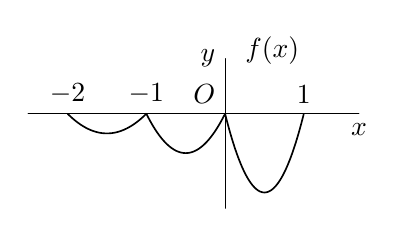
\begin{tikzpicture}[line cap=round,line join=round,scale=1]
      \draw[\myaxisarrow] (-2.5,0) -- (1.7,0) node[below] {$x$};
      \draw[\myaxisarrow] (0,-1.2) -- (0,0.7) node[left] {$y$};
      \draw[line width=0.6pt,smooth,samples=100] 
        plot[domain=-2:-1](\x,{(\x+2)*(\x+1)})
        plot[domain=-1:0](\x,{2*\x*(\x+1)})
        plot[domain=0:1](\x,{4*\x*(\x-1)});
      \draw (0,0) node[anchor=south east] {$O$} 
        (-2,0) node[above] {$-2$} (-1,0) node[above] {$-1$}
        (1,0) node[above] {$1$} (0.6,0.8) node {$f(x)$};
    \end{tikzpicture}\end{center}}
    而 $x\in[-2,-1]$ 时, $x+2\in[0,1]$, 由 $f(x+2)=4f(x)$ 知 $f_{\min}=-\frac14$.
    
    方法二: $x\in[-2,-1]$ 时, $x+2\in[0,1]$, 由 $f(x+2)=4f(x)$ 知 
    \[f(x)=\frac14 f(x+2)=(x+2)(x+1),\]
    所以 $f_{\min}= f\Bigl(-\frac32\Bigr)= -\frac14$.
  \endsolution
  
  \begin{exercise}
    已知二次函数 $f(x)=ax^2 +bx$ ($a$, $b$ 为常数, 且 $a\neq 0$) 
    满足条件 $f(x+1)=f(1-x)$, 且 $f(x)$ 的图象与直线 $y=2x$ 仅有一个公共点. 求 $f(x)$的解析式.
  \end{exercise}
  
  \beginsolution
    轴 $x=1$ 且 $ax^2+bx=2x$ 有两相等实根, 
    \mymarginpar{$f(x)$ 的图象与直线 $y=2x$ 已有公共点 $(0,0)$, 则 $y=2x$ 为 $f(x)$ 在 $(0,0)$ 处的切线, 所以 $f'(0)=2$.}
    解得 $a=1$, $b=2$, 则 $f(x)=x^2+2x$.
  \endsolution
  
%%%%%%%%%%%%%%%%%%%%%%%